% Module A: Welcome + Intro
% INStats Causal Roadmaps with AI workshop
% August 5, 2026 | all times Eastern
\documentclass[aspectratio=169]{beamer}
%%%%%%%%%%%%%%%%%%%%%%%%%%%%%%%%%%%%%%%%%%%%%%%%%%%%%%%%%%%%%%%%%%%%%%
% Shared Instats preamble for the Aug 5 segment decks.
% January template: metropolis, accent 4A9EFF, InStats_RWL.png logo.
% Each segment deck does:
%   \documentclass[aspectratio=169]{beamer}
%   %%%%%%%%%%%%%%%%%%%%%%%%%%%%%%%%%%%%%%%%%%%%%%%%%%%%%%%%%%%%%%%%%%%%%%
% Shared Instats preamble for the Aug 5 segment decks.
% January template: metropolis, accent 4A9EFF, InStats_RWL.png logo.
% Each segment deck does:
%   \documentclass[aspectratio=169]{beamer}
%   %%%%%%%%%%%%%%%%%%%%%%%%%%%%%%%%%%%%%%%%%%%%%%%%%%%%%%%%%%%%%%%%%%%%%%
% Shared Instats preamble for the Aug 5 segment decks.
% January template: metropolis, accent 4A9EFF, InStats_RWL.png logo.
% Each segment deck does:
%   \documentclass[aspectratio=169]{beamer}
%   \input{instats-preamble}
%   \title{...}\subtitle{...}\author{...}\date{...}
% and opens with \instatstitle.
%
% Placeholder types:
%   \pendingbox{owner}{what}  - content someone still owes
%   \shotslot{name}{desc}     - screenshot to capture (drop at art/<name>.png)
%   \artslot{name}{desc}      - hand-drawn art (drop at art/<name>.png)
%   \pnum{...}                - inline pending numbers/facts
%%%%%%%%%%%%%%%%%%%%%%%%%%%%%%%%%%%%%%%%%%%%%%%%%%%%%%%%%%%%%%%%%%%%%%

\usetheme{metropolis}
\usefonttheme{professionalfonts}
\usepackage[utf8]{inputenc}
\usepackage{amsmath, amssymb, mathtools, bm}
\usepackage{graphicx}
\usepackage{booktabs}
\usepackage{lmodern}
\usepackage{microtype}
\usepackage{xcolor}
\usepackage{hyperref}
\usepackage[absolute,overlay]{textpos}
\usepackage{tikz}
\usetikzlibrary{positioning,arrows.meta,shapes.geometric,calc}

\definecolor{accent}{HTML}{4A9EFF}
\definecolor{pendorange}{HTML}{E67E22}
\setbeamercolor{structure}{fg=accent}
\setbeamercolor{background canvas}{bg=white}
\metroset{progressbar=frametitle,block=fill}
\setbeamertemplate{navigation symbols}{}
\setbeamertemplate{footline}{}

\newcommand{\instatstitle}{%
  \begin{frame}[plain]
    \titlepage
    \begin{textblock*}{3cm}(11.5cm,0.5cm)
      
\includegraphics[width=3cm]{art/InStats_RWL.png}
    \end{textblock*}
  \end{frame}}

\newcommand{\pendingbox}[2]{%
  \begin{center}
  \begin{tikzpicture}
    \node[draw=pendorange, dashed, very thick, rounded corners, fill=pendorange!8,
          minimum width=0.88\textwidth, minimum height=0.52\textheight,
          align=center, text width=0.78\textwidth]
      {{\color{pendorange}\bfseries PLACEHOLDER \textbar\ owner: #1}\\[6pt] #2};
  \end{tikzpicture}
  \end{center}}

\newcommand{\shotslot}[2]{%
  \IfFileExists{art/#1.png}{%
    \begin{center}\includegraphics[height=0.62\textheight]{art/#1.png}\end{center}%
  }{%
    \begin{center}
    \begin{tikzpicture}
      \node[draw=accent, dashed, very thick, rounded corners, fill=accent!6,
            minimum width=0.88\textwidth, minimum height=0.55\textheight,
            align=center, text width=0.78\textwidth]
        {{\color{accent}\bfseries SCREENSHOT}\\[1pt] {\ttfamily art/#1.png}\\[6pt] #2};
    \end{tikzpicture}
    \end{center}}}

\newcommand{\artslot}[3][0.55]{%
  \IfFileExists{art/#2.png}{%
    \begin{center}\includegraphics[height=#1\textheight]{art/#2.png}\end{center}%
  }{%
    \begin{center}
    \begin{tikzpicture}
      \node[draw=accent, dashed, very thick, rounded corners, fill=white,
            minimum width=0.85\textwidth, minimum height=#1\textheight,
            align=center, text width=0.75\textwidth]
        {{\color{accent}\bfseries HAND-DRAWN ART}\\[1pt] {\ttfamily art/#2.png}\\[6pt] #3};
    \end{tikzpicture}
    \end{center}}}

\newcommand{\pnum}[1]{\textcolor{pendorange}{\textbf{[PENDING: #1]}}}

%   \title{...}\subtitle{...}\author{...}\date{...}
% and opens with \instatstitle.
%
% Placeholder types:
%   \pendingbox{owner}{what}  - content someone still owes
%   \shotslot{name}{desc}     - screenshot to capture (drop at art/<name>.png)
%   \artslot{name}{desc}      - hand-drawn art (drop at art/<name>.png)
%   \pnum{...}                - inline pending numbers/facts
%%%%%%%%%%%%%%%%%%%%%%%%%%%%%%%%%%%%%%%%%%%%%%%%%%%%%%%%%%%%%%%%%%%%%%

\usetheme{metropolis}
\usefonttheme{professionalfonts}
\usepackage[utf8]{inputenc}
\usepackage{amsmath, amssymb, mathtools, bm}
\usepackage{graphicx}
\usepackage{booktabs}
\usepackage{lmodern}
\usepackage{microtype}
\usepackage{xcolor}
\usepackage{hyperref}
\usepackage[absolute,overlay]{textpos}
\usepackage{tikz}
\usetikzlibrary{positioning,arrows.meta,shapes.geometric,calc}

\definecolor{accent}{HTML}{4A9EFF}
\definecolor{pendorange}{HTML}{E67E22}
\setbeamercolor{structure}{fg=accent}
\setbeamercolor{background canvas}{bg=white}
\metroset{progressbar=frametitle,block=fill}
\setbeamertemplate{navigation symbols}{}
\setbeamertemplate{footline}{}

\newcommand{\instatstitle}{%
  \begin{frame}[plain]
    \titlepage
    \begin{textblock*}{3cm}(11.5cm,0.5cm)
      
\includegraphics[width=3cm]{art/InStats_RWL.png}
    \end{textblock*}
  \end{frame}}

\newcommand{\pendingbox}[2]{%
  \begin{center}
  \begin{tikzpicture}
    \node[draw=pendorange, dashed, very thick, rounded corners, fill=pendorange!8,
          minimum width=0.88\textwidth, minimum height=0.52\textheight,
          align=center, text width=0.78\textwidth]
      {{\color{pendorange}\bfseries PLACEHOLDER \textbar\ owner: #1}\\[6pt] #2};
  \end{tikzpicture}
  \end{center}}

\newcommand{\shotslot}[2]{%
  \IfFileExists{art/#1.png}{%
    \begin{center}\includegraphics[height=0.62\textheight]{art/#1.png}\end{center}%
  }{%
    \begin{center}
    \begin{tikzpicture}
      \node[draw=accent, dashed, very thick, rounded corners, fill=accent!6,
            minimum width=0.88\textwidth, minimum height=0.55\textheight,
            align=center, text width=0.78\textwidth]
        {{\color{accent}\bfseries SCREENSHOT}\\[1pt] {\ttfamily art/#1.png}\\[6pt] #2};
    \end{tikzpicture}
    \end{center}}}

\newcommand{\artslot}[3][0.55]{%
  \IfFileExists{art/#2.png}{%
    \begin{center}\includegraphics[height=#1\textheight]{art/#2.png}\end{center}%
  }{%
    \begin{center}
    \begin{tikzpicture}
      \node[draw=accent, dashed, very thick, rounded corners, fill=white,
            minimum width=0.85\textwidth, minimum height=#1\textheight,
            align=center, text width=0.75\textwidth]
        {{\color{accent}\bfseries HAND-DRAWN ART}\\[1pt] {\ttfamily art/#2.png}\\[6pt] #3};
    \end{tikzpicture}
    \end{center}}}

\newcommand{\pnum}[1]{\textcolor{pendorange}{\textbf{[PENDING: #1]}}}

%   \title{...}\subtitle{...}\author{...}\date{...}
% and opens with \instatstitle.
%
% Placeholder types:
%   \pendingbox{owner}{what}  - content someone still owes
%   \shotslot{name}{desc}     - screenshot to capture (drop at art/<name>.png)
%   \artslot{name}{desc}      - hand-drawn art (drop at art/<name>.png)
%   \pnum{...}                - inline pending numbers/facts
%%%%%%%%%%%%%%%%%%%%%%%%%%%%%%%%%%%%%%%%%%%%%%%%%%%%%%%%%%%%%%%%%%%%%%

\usetheme{metropolis}
\usefonttheme{professionalfonts}
\usepackage[utf8]{inputenc}
\usepackage{amsmath, amssymb, mathtools, bm}
\usepackage{graphicx}
\usepackage{booktabs}
\usepackage{lmodern}
\usepackage{microtype}
\usepackage{xcolor}
\usepackage{hyperref}
\usepackage[absolute,overlay]{textpos}
\usepackage{tikz}
\usetikzlibrary{positioning,arrows.meta,shapes.geometric,calc}

\definecolor{accent}{HTML}{4A9EFF}
\definecolor{pendorange}{HTML}{E67E22}
\setbeamercolor{structure}{fg=accent}
\setbeamercolor{background canvas}{bg=white}
\metroset{progressbar=frametitle,block=fill}
\setbeamertemplate{navigation symbols}{}
\setbeamertemplate{footline}{}

\newcommand{\instatstitle}{%
  \begin{frame}[plain]
    \titlepage
    \begin{textblock*}{3cm}(11.5cm,0.5cm)
      
\includegraphics[width=3cm]{art/InStats_RWL.png}
    \end{textblock*}
  \end{frame}}

\newcommand{\pendingbox}[2]{%
  \begin{center}
  \begin{tikzpicture}
    \node[draw=pendorange, dashed, very thick, rounded corners, fill=pendorange!8,
          minimum width=0.88\textwidth, minimum height=0.52\textheight,
          align=center, text width=0.78\textwidth]
      {{\color{pendorange}\bfseries PLACEHOLDER \textbar\ owner: #1}\\[6pt] #2};
  \end{tikzpicture}
  \end{center}}

\newcommand{\shotslot}[2]{%
  \IfFileExists{art/#1.png}{%
    \begin{center}\includegraphics[height=0.62\textheight]{art/#1.png}\end{center}%
  }{%
    \begin{center}
    \begin{tikzpicture}
      \node[draw=accent, dashed, very thick, rounded corners, fill=accent!6,
            minimum width=0.88\textwidth, minimum height=0.55\textheight,
            align=center, text width=0.78\textwidth]
        {{\color{accent}\bfseries SCREENSHOT}\\[1pt] {\ttfamily art/#1.png}\\[6pt] #2};
    \end{tikzpicture}
    \end{center}}}

\newcommand{\artslot}[3][0.55]{%
  \IfFileExists{art/#2.png}{%
    \begin{center}\includegraphics[height=#1\textheight]{art/#2.png}\end{center}%
  }{%
    \begin{center}
    \begin{tikzpicture}
      \node[draw=accent, dashed, very thick, rounded corners, fill=white,
            minimum width=0.85\textwidth, minimum height=#1\textheight,
            align=center, text width=0.75\textwidth]
        {{\color{accent}\bfseries HAND-DRAWN ART}\\[1pt] {\ttfamily art/#2.png}\\[6pt] #3};
    \end{tikzpicture}
    \end{center}}}

\newcommand{\pnum}[1]{\textcolor{pendorange}{\textbf{[PENDING: #1]}}}


\title{Data Can Deceive}
\subtitle{Causal Roadmaps with AI\\[3pt]{\small Module A: Welcome + Intro}}
\author{Kathryn, Andy, Robert, and Auriane}
\institute{INStats Live Seminar}
\date{August 5, 2026 \quad \(\cdot\) \quad 12:00--12:20 ET}

% Small, editable additions to the shared INStats Beamer class.
\newcommand{\moduletime}[2]{%
  \begin{textblock*}{4.8cm}(10.65cm,0.20cm)
    \raggedleft\color{white}\fontsize{8}{9}\selectfont
    Module #1 \(\cdot\) #2 ET
  \end{textblock*}}

\newcommand{\modulefooter}[1]{%
  \begin{textblock*}{7.0cm}(0.65cm,8.62cm)
    \color{black!55}\fontsize{6.5}{7}\selectfont #1
  \end{textblock*}
  \begin{textblock*}{5.0cm}(10.35cm,8.62cm)
    \raggedleft\color{black!55}\fontsize{6.5}{7}\selectfont
    INStats \(\cdot\) August 5, 2026
  \end{textblock*}}

\newcommand{\sourcesnote}[2]{%
  \note{#1\par\medskip [Sources]\par #2}}

\newcommand{\introframe}[7]{%
  \begin{frame}{#1}
    \moduletime{A}{12:00--12:20}
    \begin{columns}[T,onlytextwidth]
      \begin{column}{0.35\textwidth}
        \centering
        \vspace{0.25cm}
        \begin{tikzpicture}
          \clip (0,0) circle (1.75cm);
          \node[inner sep=0pt] at (0,0)
            {\includegraphics[width=4.35cm]{#4}};
        \end{tikzpicture}\\[-1pt]
        {\color{accent}\rule{4.0cm}{1.2pt}}
      \end{column}
      \begin{column}{0.61\textwidth}
        \vspace{0.18cm}
        {\color{accent}\Large\bfseries #2}\par
        \vspace{0.35cm}
        {\large\bfseries #3}\par
        \vspace{0.72cm}
        {\fontsize{16}{21}\selectfont\color{black!68}#5}\par
        \vspace{0.70cm}
        {\fontsize{16}{21}\selectfont #6}
      \end{column}
    \end{columns}
    \modulefooter{Module A \(\cdot\) Welcome + Intro}
    \sourcesnote{#7}{%
      \texttt{\detokenize{intros/bios.txt}}\par
      \texttt{\detokenize{#4}}\par
      \texttt{\detokenize{planning/Workshop Outline.docx}}}
  \end{frame}}

\newcommand{\modulepreview}[5]{%
  \begin{frame}{#2}
    \moduletime{#1}{#3}
    \begin{columns}[T,onlytextwidth]
      \begin{column}{0.12\textwidth}
        \vspace{0.35cm}
        {\fontsize{54}{56}\selectfont\bfseries\color{accent!17}#1}
      \end{column}
      \begin{column}{0.025\textwidth}
        \vspace{0.25cm}
        {\color{accent}\rule{1.4pt}{4.75cm}}
      \end{column}
      \begin{column}{0.80\textwidth}
        \vspace{0.08cm}
        {\fontsize{16}{20}\selectfont
        \begin{itemize}
          \setlength{\itemsep}{0.34cm}
          \setlength{\topsep}{0.08cm}
          #4
        \end{itemize}}
        #5
      \end{column}
    \end{columns}
    \modulefooter{Module #1 \(\cdot\) #2}
    \sourcesnote{Preview the purpose and sequence of Module #1.}{%
      \texttt{\detokenize{planning/Workshop Outline.docx}}}
  \end{frame}}

\begin{document}

% 1. Welcome
\begin{frame}[plain]
  \begin{textblock*}{3cm}(11.5cm,0.5cm)
    
\includegraphics[width=3cm]{art/InStats_RWL.png}
  \end{textblock*}
  \begin{textblock*}{10cm}(1.0cm,1.80cm)
    {\fontsize{23}{26}\selectfont\bfseries Data Can Deceive}
  \end{textblock*}
  \begin{textblock*}{10cm}(1.0cm,2.75cm)
    {\fontsize{15}{18}\selectfont Causal Roadmaps with AI}
  \end{textblock*}
  \begin{textblock*}{10cm}(1.0cm,3.45cm)
    {\fontsize{12}{15}\selectfont Module A: Welcome + Intro}
  \end{textblock*}
  \begin{tikzpicture}[remember picture,overlay]
    \draw[pendorange,line width=0.6pt]
      ([xshift=1.0cm,yshift=-4.52cm]current page.north west) --
      ([xshift=-1.0cm,yshift=-4.52cm]current page.north east);
  \end{tikzpicture}
  \begin{textblock*}{10cm}(1.0cm,5.42cm)
    {\fontsize{11}{14}\selectfont Kathryn, Andy, Robert, and Auriane}
  \end{textblock*}
  \begin{textblock*}{10cm}(1.0cm,6.12cm)
    {\fontsize{11}{14}\selectfont
      August 5, 2026 \quad \(\cdot\) \quad 12:00--12:20 ET}
  \end{textblock*}
  \begin{textblock*}{10cm}(1.0cm,6.86cm)
    {\fontsize{10}{12}\selectfont INStats Live Seminar}
  \end{textblock*}
  \sourcesnote{Welcome participants and confirm that all workshop times shown
    in this deck are Eastern Time.}{%
    \texttt{\detokenize{art/InStats_RWL.png}}\par
    \texttt{\detokenize{planning/Workshop Outline.docx}}}
\end{frame}

% 2--5. Introductions
\introframe
  {Kathryn Morrison}
  {PhD \(\cdot\) PStat}
  {Co-founder and President, Precision Analytics}
  {intros/Kathryn Morrison.jpg}
  {Accredited statistician with more than twenty peer-reviewed publications.
   Her consulting spans genomics, clinical research, and statistical technology.}
  {\textbf{In this workshop:} opening context, causal foundations,
   audit-first AI, and calibration of the conclusions.}
  {Introduce Kathryn and connect her consulting experience to the opening
   discussion of why polished analyses can still fail.}

\introframe
  {Andy Wilson}
  {PhD \(\cdot\) MStat}
  {Adjunct Professor, University of Utah}
  {intros/Andy Wilson.jpg}
  {Teaches Causal Methods in Public Health and co-develops the open-source
   Causal Navigator through Tao of RWD.}
  {\textbf{In this workshop:} the causal roadmap, live Navigator
   demonstration, and TMLE walkthrough.}
  {Introduce Andy's focus on practical causal methods and the Causal Navigator.}

\introframe
  {Robert Platt}
  {PhD}
  {Professor of Biostatistics, McGill University}
  {intros/Robert Platt.jpg}
  {Co-lead of the Canadian Network for Observational Drug Effect Studies
   (CNODES), with a focus on pharmacoepidemiology using claims and EHR data.}
  {\textbf{In this workshop:} a concrete example of why the causal roadmap matters.}
  {Introduce Robert's example as the handoff from the welcome into the
   substantive workshop.}

\introframe
  {Auriane Journet}
  {MScPH student}
  {McGill University \(\cdot\) President, UAEM McGill}
  {intros/Auriane Journet.jpg}
  {Auriane supports the workshop's live delivery.}
  {\textbf{In this workshop:} screen share and production support,
   including the live Navigator session.}
  {Introduce Auriane and clarify her visible role in the live Navigator session.}

% 6. Opening prompt
\begin{frame}{Before we begin}
  \moduletime{A}{12:00--12:20}
  \begin{center}
    \vspace{0.70cm}
    {\color{accent}\large\bfseries Chat prompt}\par
    \vspace{0.65cm}
    {\LARGE\itshape Which step in your current study\\
      feels least defensible?}\par
    \vspace{0.95cm}
    {\large\color{black!60} Add one step or decision in the chat.}
  \end{center}
  \modulefooter{Module A \(\cdot\) Welcome + Intro}
  \sourcesnote{Collect several answers. Return to them in Module H.}{%
    \texttt{\detokenize{SegmentA_Welcome.tex}}\par
    \texttt{\detokenize{planning/Workshop Outline.docx}}}
\end{frame}

% 7. Visual journey through the day
\begin{frame}[plain]
  \begin{tikzpicture}[remember picture,overlay]
    \node[anchor=south west,inner sep=0pt] at (current page.south west)
      {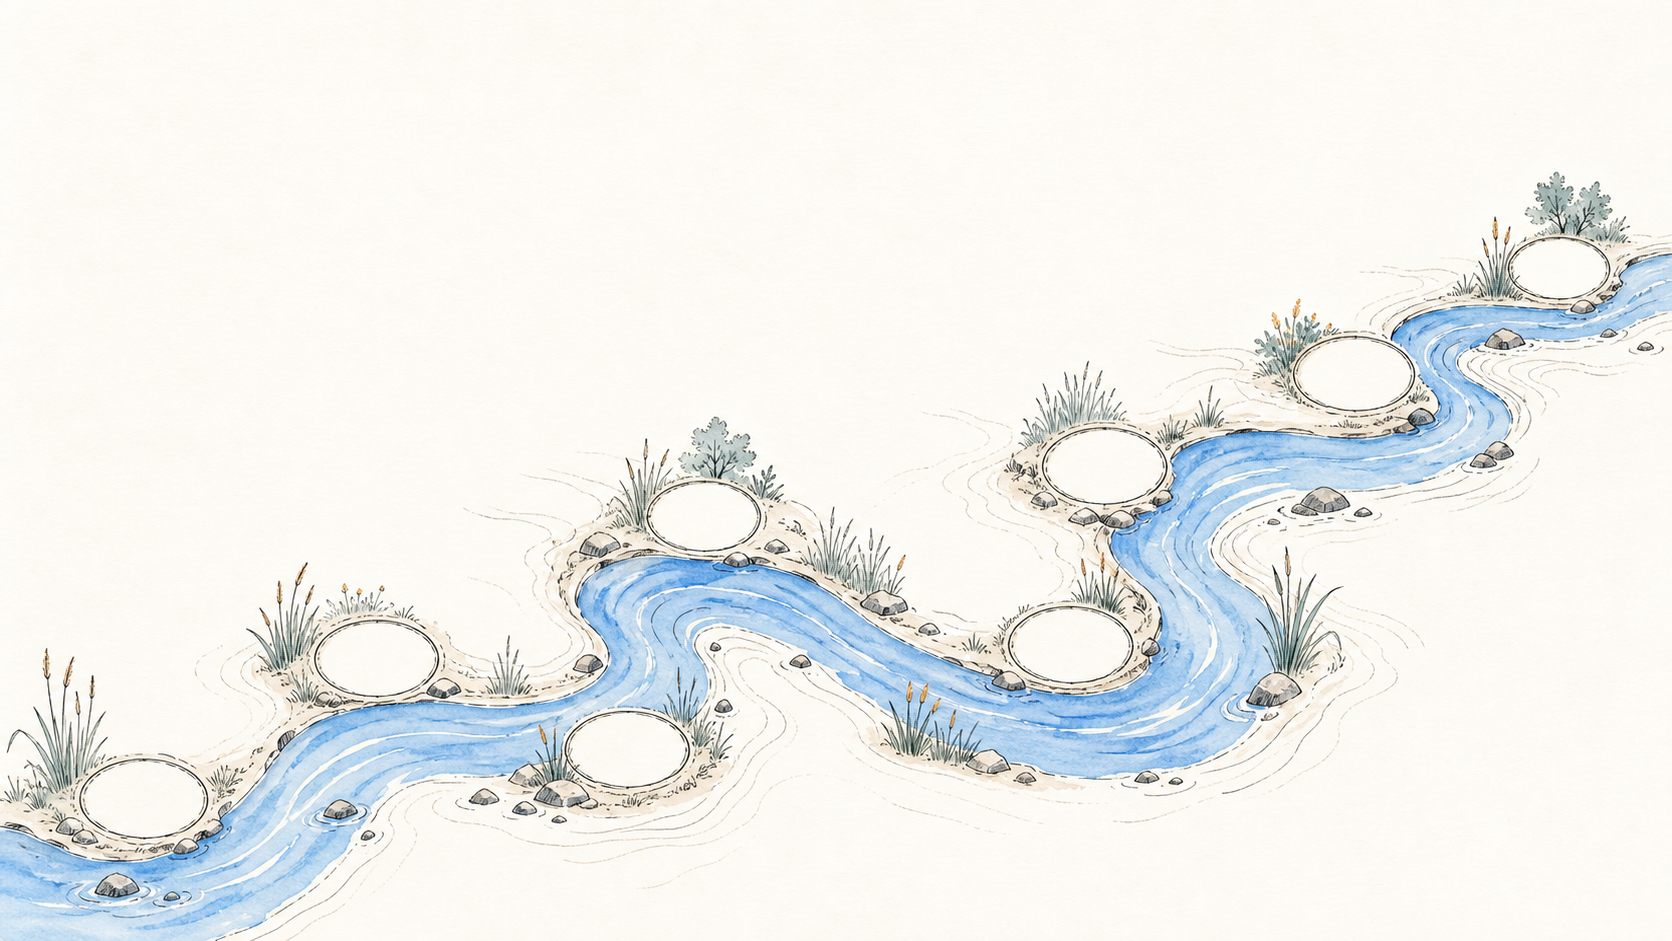
\includegraphics[width=\paperwidth,height=\paperheight]{art/river-journey.png}};

    \fill[white,opacity=0.92]
      (current page.north west) rectangle
      ([yshift=-1.45cm]current page.north east);

    \node[anchor=north west,text=black!82,font=\bfseries\fontsize{22}{24}\selectfont]
      at ([xshift=0.55cm,yshift=-0.24cm]current page.north west)
      {Workshop journey \(\cdot\) 12:00--5:00 ET};

    \node[anchor=north west,text=black!62,font=\fontsize{9.2}{11}\selectfont]
      at ([xshift=0.56cm,yshift=-0.94cm]current page.north west)
      {A Welcome \quad B Robert \quad C Foundations \quad D Roadmap \quad
       E AI audit \quad F Navigator \quad G TMLE \quad H Close};

    % The underlying illustration contains eight blank stopping places.
    \foreach \letter/\x/\y in {
      A/1.20/7.49,
      B/3.59/6.21,
      C/5.89/7.15,
      D/6.73/4.94,
      E/10.23/6.16,
      F/10.60/4.46,
      G/12.75/3.53,
      H/15.01/2.56}
      \node[font=\bfseries\fontsize{18}{20}\selectfont,text=black!82]
        at ([xshift=\x cm,yshift=-\y cm]current page.north west) {\letter};

    \node[anchor=north west,fill=white,fill opacity=0.86,text opacity=1,
          rounded corners=2pt,inner sep=3pt,font=\itshape\fontsize{8.5}{10}\selectfont]
      at ([xshift=5.80cm,yshift=-7.52cm]current page.north west)
      {Break \(\cdot\) 1:25--1:35 ET};
    \node[anchor=north west,fill=white,fill opacity=0.86,text opacity=1,
          rounded corners=2pt,inner sep=3pt,font=\itshape\fontsize{8.5}{10}\selectfont]
      at ([xshift=8.60cm,yshift=-6.80cm]current page.north west)
      {Lunch \(\cdot\) 2:45--3:15 ET};
    \node[anchor=north west,fill=white,fill opacity=0.86,text opacity=1,
          rounded corners=2pt,inner sep=3pt,font=\itshape\fontsize{8.5}{10}\selectfont]
      at ([xshift=11.18cm,yshift=-4.86cm]current page.north west)
      {Break \(\cdot\) 4:10--4:20 ET};
  \end{tikzpicture}
  \sourcesnote{Use the river as a quick visual overview. The next seven slides
    preview Modules B through H.}{%
    \texttt{\detokenize{art/river-journey.png}}\par
    \texttt{\detokenize{planning/Workshop Outline.docx}}}
\end{frame}

% 8--14. One preview slide per remaining module
\modulepreview{B}{Example with Robert Platt}{12:20--12:45}{
  \item The research question
  \item What looked persuasive
  \item What went wrong---and the consequence
  \item Where the failure sits in the eight-step Navigator
}{}

\modulepreview{C}{Foundations}{12:45--1:25}{
  \item Association versus intervention
  \item Counterfactual contrasts; confounders, mediators, and colliders
  \item Target-trial protocol and time-zero alignment
  \item Pneumonia-vaccine example and its crude paradox
}{}

\modulepreview{D}{The Roadmap}{1:35--2:20}{
  \item Protocol: population, strategies, time zero, follow-up, outcome, contrast
  \item DAG: measured and unmeasured common causes
  \item Observed-data mapping and identification assumptions
  \item Estimand, estimator, sensitivity plan, and interpretation
}{}

\modulepreview{E}{Audit-First AI}{2:20--2:45}{
  \item Review an AI-generated roadmap field
  \item Accept, correct, or reject it
  \item Name the evidence required
  \item Record the decision in the audit log
}{}

\modulepreview{F}{Live Navigator}{3:15--4:10}{
  \item Start from Quick Start using the no-login manual route
  \item Complete eight steps from prepared entries
  \item Use AI Copilot once, if the presenter account is ready
  \item Export the study summary
}{%
  \vspace{0.12cm}
  {\color{accent}\fontsize{11}{14}\selectfont\bfseries
   Discussion pauses: treatment strategy \(\cdot\) unmeasured confounding
   \(\cdot\) interpretation}}

\modulepreview{G}{TMLE}{4:20--4:55}{
  \item Start from the estimand already defined in Navigator
  \item Compare crude, g-computation, IPW, and TMLE estimates
  \item Review the outcome model, treatment model, and targeting update
  \item Inspect overlap and state what TMLE cannot repair
}{}

\modulepreview{H}{Close + Kit}{4:55--5:00}{
  \item Protocol \(\cdot\) roadmap \(\cdot\) audit \(\cdot\) estimation
        \(\cdot\) interpretation
  \item Participant workshop kit
  \item Right-heart-catheterization worked example
  \item Exit question: What will you change before your next model is fit?
}{}

\end{document}
